% Compile from this directory: tectonic Reinforcement_2D_Shooter_IEEE_Report.tex
% Or: latexmk -pdf Reinforcement_2D_Shooter_IEEE_Report.tex
% Author order: Minh Quan Dinh, then Quoc Anh Phan.
\documentclass[conference]{IEEEtran}
\usepackage[T1]{fontenc}
\usepackage{amsmath,amssymb}
\usepackage{graphicx}
\usepackage{booktabs,tabularx,array}
\usepackage{xcolor}
\usepackage{tikz}
\usetikzlibrary{arrows.meta,positioning,calc}
\usepackage{listings}
\usepackage{cite}
\usepackage[hidelinks]{hyperref}
\urlstyle{same}
\graphicspath{{figures/}}
\definecolor{reportblue}{HTML}{176394}
\lstset{basicstyle=\ttfamily\scriptsize,breaklines=true,columns=fullflexible,
  keepspaces=true,showstringspaces=false,frame=single,rulecolor=\color{black!25},
  xleftmargin=3pt,xrightmargin=3pt,aboveskip=7pt,belowskip=7pt}
\newcommand{\code}[1]{\texttt{\detokenize{#1}}}
\newcommand{\E}{\mathbb{E}}
\newcommand{\R}{\mathbb{R}}
\newcolumntype{Y}{>{\raggedright\arraybackslash}X}
\interdisplaylinepenalty=2500
\begin{document}

\title{PPO for a Partially Observable 2D Shooter:\\Bullet-Set Encoding and Bounded Temporal Policies}
\author{\IEEEauthorblockN{Minh Quan Dinh, Quoc Anh Phan}}
\maketitle

\begin{abstract}
This paper investigates bounded observation history for reinforcement learning in a partially observable 2D shooter. The agent receives local wall distances, angular enemy detections, body state, previous actions, and a variable number of visible hostile projectiles. A permutation-invariant set encoder summarizes the projectiles, and Proximal Policy Optimization trains a feedforward actor--critic or a policy augmented with LSTM/BiLSTM context. A five-stage curriculum increases opponent mobility, spawning difficulty, and evasion. In a matched experiment, a randomly initialized BiLSTM and feedforward control each receive 2,769,992 environment transitions under the same PPO configuration and training seed. The BiLSTM completes all five curriculum stages, whereas the control completes stages 0--2. Across 24 held-out stage-4 trials, combat success is 100.0\% versus 66.7\%, and mean episodic return is 44.17 versus 22.67. The paired success difference is 33.3 percentage points, with a 95\% bootstrap interval of [16.7,54.2]. Restricting the trained BiLSTM to the current observation lowers mean return to 28.92, although its success-difference interval includes zero. These findings motivate further study of temporal context, subject to the single-training-seed design, increased model capacity, and higher computational cost.
\end{abstract}

\begin{IEEEkeywords}
reinforcement learning, proximal policy optimization, partial observability, Deep Sets, bidirectional LSTM, curriculum learning, game agents
\end{IEEEkeywords}

\section{Introduction}
A shooter agent must coordinate navigation and combat under incomplete information. Walls provide cover but also hide targets, incoming projectiles demand rapid responses, and aiming competes with scanning for new threats. A useful training environment should expose these interactions while allowing repeatable experiments and inspection of learned behavior.

We study this problem in a custom 800$\times$800 arena with PyTorch policies, Gymnasium episode semantics, and a Pygame front end~\cite{repository}. Policies act on compact numerical features. The system combines Proximal Policy Optimization (PPO)~\cite{ppo}, a set encoder inspired by Deep Sets~\cite{deepsets}, and optional LSTM context~\cite{lstm}. A shared trainer supports comparisons between feedforward and recurrent policies under a common environment and optimization procedure.

The main experimental question is whether a short observation history helps a policy cope with occlusion and temporal ambiguity under a matched interaction budget. A second question is whether the trained recurrent policy depends on that history at inference. These questions require different comparisons: scratch feedforward versus scratch BiLSTM measures the architecture change under the recorded training procedure, while a history ablation tests the sensitivity of one trained policy to its temporal input.

The contributions are an integrated combat environment with angular sensing and variable-cardinality projectile inputs, a shared PPO pipeline for feedforward and recurrent policies, and a matched-budget evaluation with held-out maps and history ablation. The study evaluates this combination of established methods within the implemented environment, with its architectural claims limited by training-seed count and model capacity.

\section{Related Work}
PPO optimizes a clipped policy surrogate using multiple minibatch passes over recently collected experience~\cite{ppo}. Generalized Advantage Estimation (GAE) combines value estimates and temporal-difference residuals to control the bias--variance tradeoff in policy-gradient learning~\cite{gae}. We use these established optimization components for all compared policies, keeping the learning objective fixed while changing temporal context.

LSTM provides a gated recurrent architecture for sequence processing~\cite{lstm}. Hausknecht and Stone investigate recurrent Q-learning under partial observability and show that integrating observations through time can improve adaptation when observability changes~\cite{drqn}. Their results also caution against assuming that recurrence systematically improves every task. Our study instead uses PPO, local geometric observations, and a finite raw-observation window that is recomputed during optimization. Both directions of the BiLSTM operate only on observations available at action time.

Deep Sets develops neural representations whose outputs are invariant to the order of set elements~\cite{deepsets}. We apply shared per-element features and symmetric pooling to visible projectiles. This addresses changing projectile count and arbitrary ordering without requiring a fixed list size. Curriculum learning organizes experience from simpler to more difficult cases~\cite{curriculum}. Here, progression uses explicit combat stages and recent performance, with replay of earlier stages. Because both architectures share that adaptive curriculum, their learned trajectories and stage exposure can still differ.

\section{Environment and Problem Formulation}
\subsection{Partially Observable Interaction}
The interaction follows a partially observable Markov decision process $(\mathcal{S},\mathcal{A},\mathcal{O},P,Z,R,\gamma)$. Here $P$ governs transitions, $Z$ produces observations, and $R$ defines reward. Let $s_t$ denote the complete simulator state, including bodies, projectiles, obstacles, and opponent behavior. The agent receives only $o_t=g(s_t)\in\mathcal{O}$ and selects an action $a_t$. Its objective is
\begin{equation}
J(\theta)=\E_{\pi_\theta}\!\left[\sum_{t=0}^{T-1}\gamma^t r_t\right].
\end{equation}
The policy conditions on either the current observation or a finite window $H_t=(o_{\max(0,t-L+1)},\ldots,o_t)$ within the current episode. The environment is partially observable because the policy cannot access the full map, absolute coordinates, hidden projectiles, explicit target velocity, curriculum stage, or remaining episode time. The simulator retains these quantities internally.

The default time step is $1/30$\,s, and the episode limit is 1,000 steps, approximately 33.3\,s. In scripted combat, death terminates the episode and reaching the limit truncates it. A defeated target respawns within the same episode. Accordingly, this task rewards repeated hunting and survival rather than a native win condition.

The simulator also supports passive hunting, in which the target does not shoot and episodes end at the time limit, and symmetric self-play duels. Interactive human control supports demonstrations and inspection. The reported architecture comparison uses scripted combat with shooting opponents throughout.

\subsection{Map Generation and Dynamics}
Generated maps divide the interior of the arena into nine slots and select six to nine slots without replacement. Each selected slot receives one rectangular obstacle with width and height sampled between 40 and 150 units. Boundary walls are 20 units thick. A 48-unit margin inside each slot leaves at least 96 units between obstacles in adjacent occupied slots and at least 48 units to boundary walls. These clearances exceed the default body diameter of 28 units. Geometry depends on a map seed, separately from spawn and action randomness.

Each worker cycles its configured maps on episode reset; target respawns preserve the current map. Explicitly resetting with a seed restarts that worker's map cycle. The default training set contains map seeds 0--9. Fig.~\ref{fig:arenas} shows actual application frames on two generated layouts.

Bodies use circular wall collision resolution with sliding. Desired movement is relative to the updated aim direction, and normalized diagonal commands avoid a speed advantage. Velocity approaches the commanded velocity through
\begin{equation}
v_{t+1}=v_t+\min(1,12\Delta t)(v_t^{\mathrm{cmd}}-v_t).
\end{equation}
The agent's maximum speed is 220 units/s and turn rate is $200^\circ$/s. The simulator does not resolve body-to-body collisions. Projectiles use swept collision checks along their travel segment and stop at the first wall, target, or remaining range, preventing fast shots from simply passing through obstacles between frames.

\begin{figure}[t]
\centering
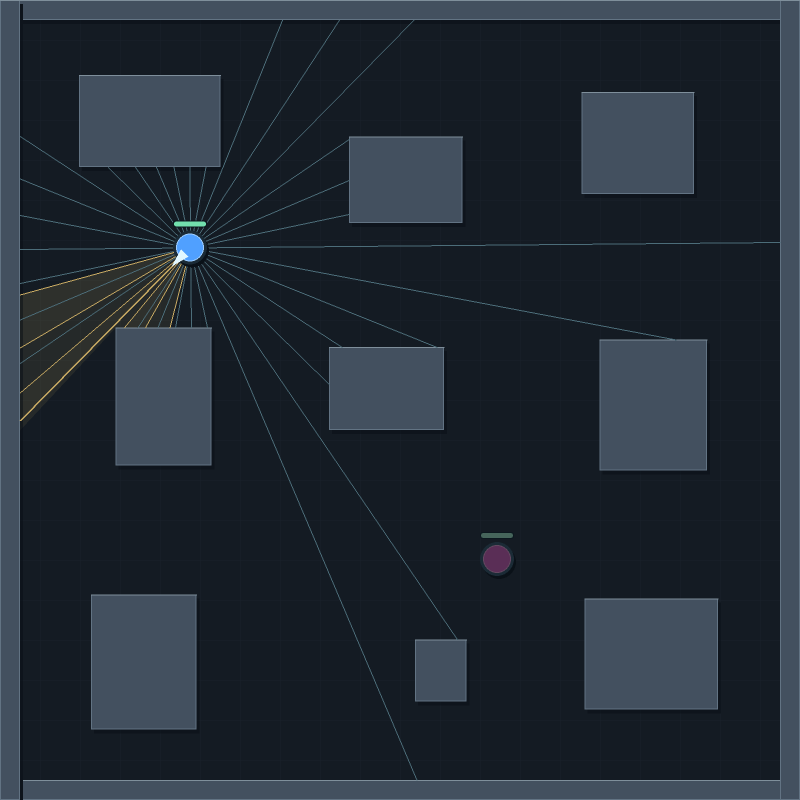
\includegraphics[width=.48\columnwidth]{arena_seed_2.png}\hfill
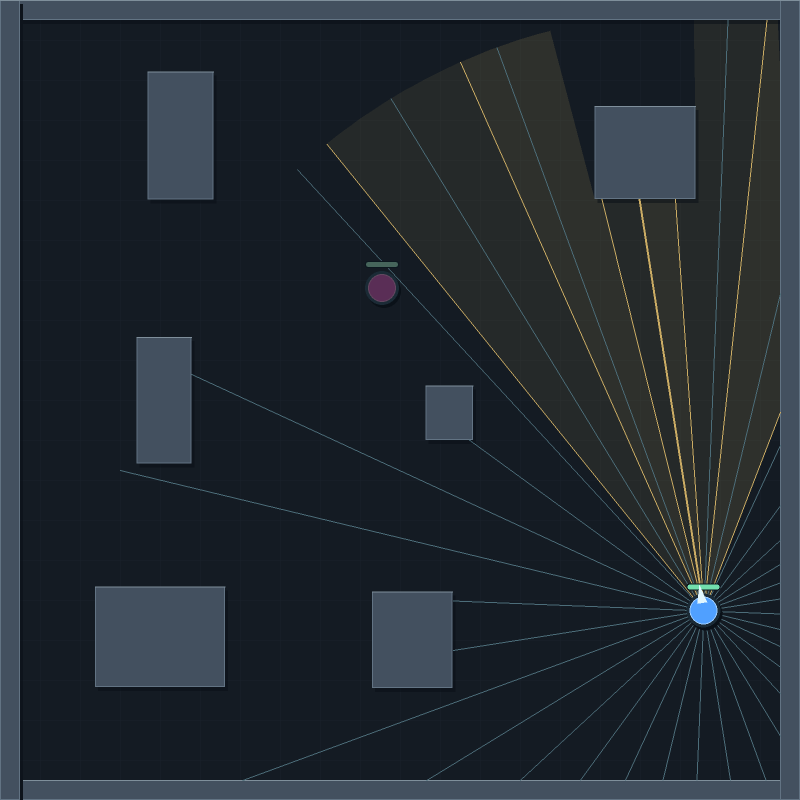
\includegraphics[width=.48\columnwidth]{arena_seed_11.png}
\caption{Actual renderer frames on map seeds 2 and 11 with angular sensing enabled. Walls constrain motion, sight, and shots. Overlays aid inspection and do not add information to the policy. These are illustrative initial states, not performance measurements.}
\label{fig:arenas}
\end{figure}

\subsection{Weapons and Opponents}
Both fighters have 100 health, and each projectile deals 25 damage. Agent shots travel at 900 units/s with a range of 900 units and a 0.35\,s firing cooldown. The scripted opponent fires toward the agent when line of sight and range permit, using speed 450 units/s, range 600 units, and cooldown 0.8\,s. The cooldown and frame interval discretize the actual firing schedule.

The scripted target navigates between sampled waypoints, uses short wall rays for avoidance, and can strafe when the agent aims near it. A stationary stage-0 opponent can still shoot. On a kill, the environment clears friendly bullets and respawns the target; hostile bullets already in flight remain active. Thus, killing a target does not remove an existing threat to survival.

\subsection{Action Space and Rewards}
Actions follow \code{MultiDiscrete([9,3,2])}: stay or move in eight relative directions, turn left/hold/right, and hold/fire. This gives 54 joint combinations. Three categorical heads represent the distribution as
\begin{equation}
\pi_\theta(a_t\mid H_t)=\prod_{k\in\{m,a,f\}}\pi_\theta^{(k)}(a_t^{(k)}\mid H_t).
\end{equation}
The shared network couples the decisions through its features, while the output distribution factorizes conditional on those features.

Let $h_t$ count hits, $k_t$ count kills, $w_t$ count shots created without a previously detected enemy, $d_t$ be actual health lost, and $q_t$ indicate agent death. The default combat reward is
\begin{equation}
r_t=h_t+3k_t-0.1w_t-0.04d_t-3q_t.
\label{eq:reward}
\end{equation}
Four hits defeat a full-health enemy, yielding $4+3=7$ points before penalties. Losing 25 health costs one point. Losing all health costs four points plus the death penalty. An ordinary miss against a detected enemy has no separate penalty. A fire request during cooldown creates no projectile and incurs no wasted-shot penalty. The latter uses detection from before the current action.

Optional exploration shaping rewards increases in maximum displacement from an invisible anchor while searching. It pays 0.0005 per unit up to 100 units per anchor, caps total bonus at 0.5 per episode, and resets the anchor on spawn, kills, or after five simulated seconds. Since revisits can earn rewards after a reset, this measures travel rather than map novelty. The primary matched experiment disables this option.

\section{Observation Representation}
\subsection{Angular State}
The default state vector contains 64 values, detailed in Table~\ref{tab:observation}. Thirty-two rays measure walls around the body with a 600-unit limit. Enemy sensing covers a forward $60^\circ$ cone divided at $-30,-15,-5,0,5,15,30$ degrees. Each sector records presence and the nearest visible target-surface distance. The algorithm considers target silhouettes and partitions visibility around wall corners, reducing the blind gaps of the older five-ray enemy sensor. A separate center ray supplies alignment information without restricting firing. The original trainer retains a legacy 60-value state based on five enemy rays; both policies in the primary study use the 64-value angular state and projectile sensing.

\begin{table}[t]
\caption{Default Angular State Layout (Zero-Based Indices)}
\label{tab:observation}
\centering\footnotesize
\begin{tabularx}{\columnwidth}{@{}l r Y@{}}
\toprule
Indices & Count & Meaning \\
\midrule
0--31 & 32 & Wall distances divided by 600 \\
32--37 & 6 & Enemy-sector presence flags \\
38--43 & 6 & Enemy-sector distances divided by 600 \\
44--45 & 2 & Center flag and normalized distance \\
46--47 & 2 & Local velocity divided by maximum speed \\
48--49 & 2 & Normalized cooldown and health \\
50--63 & 14 & Previous movement, aim, and fire one-hot groups \\
\midrule
Total & 64 & Fixed state values \\
\bottomrule
\end{tabularx}
\end{table}

\subsection{Visible Hostile Projectile Sets}
Visible hostile bullets form a variable-length set $B_t=\{b_{t,i}\}_{i=1}^{N_t}$ with four features per bullet:
\begin{equation}
b_{t,i}=\left[\frac{\Delta p_f}{600},\frac{\Delta p_r}{600},
\frac{\Delta v_f}{u_i+220},\frac{\Delta v_r}{u_i+220}\right].
\end{equation}
Subscripts $f$ and $r$ denote forward and right components in the current agent frame; $u_i$ is the bullet speed and $\Delta v$ is relative to agent velocity. Sensing includes live hostile bullets only when their positions lie within the continuous viewing cone, range, and unoccluded line of sight. Friendly bullets are excluded.

A shared MLP $\phi:\R^4\!\to\R^{32}$, implemented as $4\to32\to32$ with Tanh activations, embeds each bullet. The summary combines masked mean and elementwise maximum with bounded cardinality:
\begin{align}
c_t &= \frac{N_t}{N_t+1},\\
z_t^B &= \rho\!\left(\left[\frac{1}{N_t}\sum_i\phi(b_{t,i}),
\max_i\phi(b_{t,i}),c_t\right]\right),
\end{align}
where $\rho$ is a $65\to32$ linear layer followed by Tanh. Empty sets explicitly produce zero summaries. This pooling is invariant to bullet order, following the set-processing principle of~\cite{deepsets}. Batching pads only to the largest set in that batch and masks absent entries; it imposes no fixed projectile-count cutoff. The complete feature vector is $x_t=[o_t^{\mathrm{state}},z_t^B]\in\R^{96}$.

\section{Policy Architectures}
\subsection{Feedforward Actor--Critic}
The baseline maps $x_t$ through two 256-unit Tanh layers shared by the actor and critic. Separate linear heads output 9 movement logits, 3 aim logits, 2 fire logits, and one scalar state-value estimate. The default angular Deep Sets model contains 97,807 trainable parameters. During training, the policy samples from each head; deterministic evaluation selects each head's argmax. Trunk and output weights use orthogonal initialization with gains $\sqrt{2}$ for hidden layers, 0.01 for actor heads, and 1 for the value head, with zero biases. The projectile encoder and LSTM retain framework defaults except for the zero memory projection.

\subsection{Bounded LSTM and BiLSTM Memory}
The recurrent policy retains the same bullet encoder, decision MLP, and output heads. It encodes a window of at most 32 feature vectors using one LSTM layer, with 48 hidden units per direction for BiLSTM. A unidirectional LSTM variant is also available, although the primary saved study compares BiLSTM with feedforward.

For BiLSTM, the concatenated final forward and backward hidden states provide a 96-value temporal representation. A learned $96\to96$ projection adds a residual correction to the current feature:
\begin{align}
m_t &= [\overrightarrow{h}_{\mathrm{final}},\overleftarrow{h}_{\mathrm{final}}],\\
\widetilde{x}_t &= x_t+W_m m_t+b_m.
\label{eq:residual}
\end{align}
Fig.~\ref{fig:architecture} summarizes the computation. The model contains 163,183 parameters, approximately 66.8\% more than the feedforward control. The memory projection starts at zero, so the initial policy uses only the current features. The first optimizer step gives no gradient to the LSTM through the zero projection; subsequent updates train it as the projection changes. All model components train jointly from random initialization in the primary study.

\begin{figure*}[t]
\centering
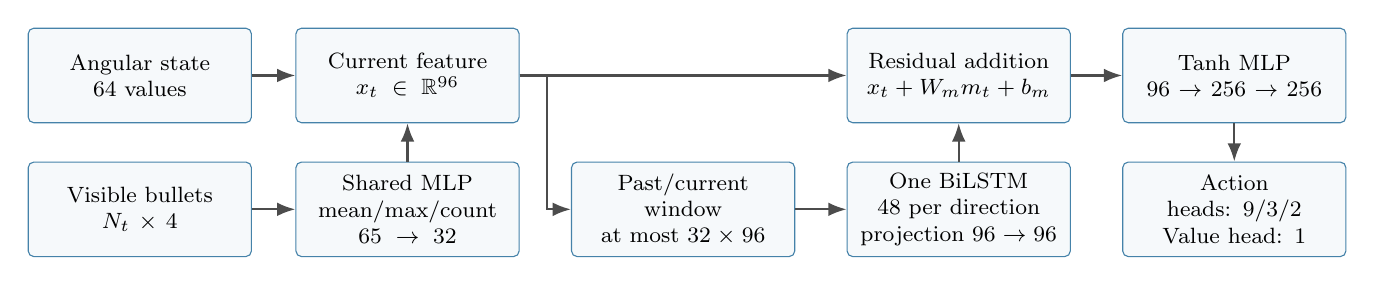
\begin{tikzpicture}[font=\footnotesize,>=Latex,
 b/.style={draw=reportblue!80,fill=reportblue!4,rounded corners=2pt,align=center,minimum height=12mm,text width=26mm},
 arr/.style={->,thick,draw=black!70}]
\node[b] (state) at (0,0) {Angular state\\64 values};
\node[b] (bullets) at (0,-1.7) {Visible bullets\\$N_t\times4$};
\node[b] (sets) at (3.4,-1.7) {Shared MLP\\mean/max/count\\$65\to32$};
\node[b] (feature) at (3.4,0) {Current feature\\$x_t\in\R^{96}$};
\node[b] (window) at (6.9,-1.7) {Past/current window\\at most $32\times96$};
\node[b] (memory) at (10.4,-1.7) {One BiLSTM\\48 per direction\\projection $96\to96$};
\node[b] (sum) at (10.4,0) {Residual addition\\$x_t+W_m m_t+b_m$};
\node[b] (mlp) at (13.9,0) {Tanh MLP\\$96\to256\to256$};
\node[b] (heads) at (13.9,-1.7) {Action heads: 9/3/2\\Value head: 1};
\draw[arr] (state)--(feature);
\draw[arr] (bullets)--(sets);
\draw[arr] (sets)--(feature);
\draw[arr] (feature)--(sum);
\draw[arr] (feature.east)--++(.35,0)|-(window.west);
\draw[arr] (window)--(memory);
\draw[arr] (memory)--(sum);
\draw[arr] (sum)--(mlp);
\draw[arr] (mlp)--(heads);
\end{tikzpicture}
\caption{Implemented BiLSTM actor--critic. Both directions process a window ending at the current observation. The feedforward control sends $x_t$ directly to the same decision MLP. Time padding and projectile padding use independent masks.}
\label{fig:architecture}
\end{figure*}

\subsection{Temporal Correctness}
Bidirectional processing occurs entirely inside the available historical window. Both directions therefore access past and current observations only; neither sees observations after the action time. The implementation concatenates both final hidden states rather than taking the last output timestep's backward component, which would summarize a different portion of the sequence.

Raw observation deques continue across rollout boundaries and clear on episode resets. They represent bounded context rather than a persistent hidden state. At 30\,Hz, 32 observations span approximately $(32-1)/30=1.03$\,s between oldest and newest samples. Each PPO minibatch recomputes complete windows with current network weights, allowing gradients through past bullet encodings and avoiding stale rollout hidden states. Packed sequences ignore time padding, while the bullet encoder independently masks projectile padding. Truncation-value estimation appends the terminal observation to the ending episode's history before that history clears.

\section{Learning Procedure}
\subsection{PPO and Generalized Advantage Estimation}
PPO alternates between collecting on-policy experience and optimizing a clipped surrogate objective~\cite{ppo}. For the joint action probability ratio
\begin{equation}
\varrho_t(\theta)=\frac{\pi_\theta(a_t\mid H_t)}{\pi_{\theta_{\mathrm{old}}}(a_t\mid H_t)},
\end{equation}
the minimized policy loss is
\begin{equation}
\mathcal{L}_{\pi}=-\E_t\!\left[\min\!\left(\varrho_t\widehat{A}_t,
\operatorname{clip}(\varrho_t,1-\epsilon,1+\epsilon)\widehat{A}_t\right)\right].
\end{equation}
Log probabilities and entropy sum over the three categorical heads. Advantages are normalized separately in each minibatch. The implementation uses
\begin{align}
\mathcal{L}_V &= \tfrac12\E_t[(V_\theta(H_t)-\widehat{R}_t)^2],\\
\mathcal{L} &= \mathcal{L}_{\pi}+0.5\mathcal{L}_V-0.01\E_t[\mathcal{H}(\pi_\theta)].
\end{align}
Thus, the explicit half factor inside $\mathcal{L}_V$ is additional to its 0.5 coefficient in the total loss. There is no value clipping or target-KL early stop; approximate KL is logged for inspection.

Generalized Advantage Estimation (GAE)~\cite{gae} recursively combines temporal-difference residuals. With $d_t$ indicating either episode boundary, the rollout implementation computes
\begin{align}
\delta_t &= \bar r_t+\gamma(1-d_t)V_{t+1}-V_t,\\
\widehat{A}_t &= \delta_t+\gamma\lambda(1-d_t)\widehat{A}_{t+1},\\
\widehat{R}_t &= \widehat{A}_t+V_t.
\end{align}
Here $\bar r_t=r_t+\gamma V(H_{t+1}^{\mathrm{terminal}})$ for a time-limit truncation without death, and $\bar r_t=r_t$ otherwise. This reward adjustment bootstraps time limits while the boundary mask prevents GAE from crossing into a reset episode. Death takes precedence if termination and truncation occur together. Logged environmental returns retain the original combat rewards, not the bootstrap adjustment.

\begin{table}[t]
\caption{Shared Training Configuration in the Primary Study}
\label{tab:hyperparameters}
\centering\footnotesize
\begin{tabularx}{\columnwidth}{@{}Y r@{}}
\toprule Parameter & Value \\
\midrule
Parallel environments / rollout steps per environment & 8 / 256 \\
Transitions per full PPO cycle & 2,048 \\
Minibatch size / epochs per rollout & 512 / 4 \\
Adam learning rate / epsilon & $3\times10^{-4}$ / $10^{-5}$ \\
Discount $\gamma$ / GAE $\lambda$ & 0.99 / 0.95 \\
PPO clipping $\epsilon$ & 0.2 \\
Value-loss / entropy coefficients & 0.5 / 0.01 \\
Maximum gradient norm & 0.5 \\
Decision hidden width & 256 \\
BiLSTM hidden units per direction / window & 48 / 32 \\
Episode horizon & 1,000 steps \\
Training seed / map seeds & 0 / 0--9 \\
Replay probability & 0.2 \\
Promotion mean reward / qualifying episodes & 35 / 100 \\
Exploration bonus / self-play & Disabled / disabled \\
Learner device & CUDA, GTX 1650 \\
\bottomrule
\end{tabularx}
\end{table}

\subsection{Parallel Collection and Training Engines}
Eight spawned CPU workers simulate independent environments. The learner batches observations, performs inference on CPU or CUDA, and sends actions back to the workers. Game simulation remains CPU work even when policy optimization uses a GPU. Default collection yields $8\times256=2,048$ transitions, four minibatches per epoch, and 16 Adam steps across four epochs. A recorded PPO update denotes this complete cycle, not an individual optimizer step.

The original trainer supports feedforward combat and self-play on CPU. The shared scratch engine supports feedforward, LSTM, and BiLSTM policies on CPU or CUDA. It shortens a final rollout to honor an exact transition budget divisible by the environment count and optimizes collected transitions in a graceful final partial rollout. The original engine can discard its last incomplete rollout at a graceful stop. The primary comparison uses the shared engine for both policies.

\subsection{Curriculum and Completion}
Table~\ref{tab:curriculum} lists the five difficulty stages. Stages 0 and 1 request visible targets near the current aim; subsequent stages broaden placement and mobility. Stage 4 prefers hidden spawns and enables aim evasion. These are requested spawn constraints: bounded sampling can relax them if a valid placement cannot be found.

\begin{table}[t]
\caption{Scripted Combat Curriculum}
\label{tab:curriculum}
\centering\footnotesize
\begin{tabularx}{\columnwidth}{@{}c r l Y@{}}
\toprule Stage & Speed & Distance & Placement / behavior \\
\midrule
0 & 0 & 80--250 & $\pm10^\circ$; line of sight \\
1 & 60 & 100--350 & $\pm30^\circ$; line of sight \\
2 & 120 & 150--500 & $\pm90^\circ$; may be occluded \\
3 & 180 & 200--700 & Any direction \\
4 & 180 & 250--900 & Prefer hidden positions; evade aim \\
\bottomrule
\end{tabularx}
\end{table}

Promotion requires the latest 100 qualifying episodes at the current stage to average at least 35 reward. Replay episodes, sampled with probability 0.2 from earlier stages, do not qualify. Promotions clear the reward window. The scratch engine additionally maintains a stage-4 window with the same threshold; reaching stage 4 alone is insufficient for all-stage completion. The primary recurrent run also requires at least 2,501,688 transitions before curriculum-based stopping. Its feedforward control instead trains to the recurrent run's final budget, regardless of mastery.

\section{System Features and Experimental Records}
\subsection{Monitoring, Checkpoints, and Resume}
A Streamlit/Plotly dashboard displays episode performance and PPO statistics through a local metrics bridge. Training can run without the dashboard. Persistent CSV files sample metrics every ten completed episodes plus a final partial sample, and an offline HTML report records configuration and stop reason. Episode metrics average up to 100 recent episodes across workers, including replay; these averages are distinct from stage qualification windows.

The scratch engine atomically saves model weights, Adam state, architecture, curriculum progress, final-stage rewards, step counters, initialization, training settings, and device information. Checkpoints store tensors on CPU for portability. Resume requires an explicit flag and matching scientific settings. It restores training progress but does not restore live simulator states or the full RNG trajectory, so continuation is not bit-for-bit identical to uninterrupted training. The original trainer automatically resumes an existing output checkpoint, making a fresh output name necessary for an independent run.

The comparison pipeline freezes a reference checkpoint and records SHA-256 identities, configuration, and archived application source. The accompanying evidence preserves raw episodes, summaries, training telemetry, and validation records, allowing the reported metrics to be traced to the evaluated policies.

\subsection{Self-Play and Interactive Inspection}
Self-play uses two identical agent bodies with the same sensing and weapon parameters. Only the blue learner supplies PPO data. The red opponent samples actions from a frozen policy refreshed every 50 PPO cycles by default. Both actions are chosen before movement, and projectile impacts are gathered before damage resolves, permitting mutual kills. First death ends a round; mutual death and timeouts are terminal draws with no continuation bootstrap. New self-play runs copy initial model weights into a separate output while preserving the source checkpoint. Curriculum replay and exploration shaping are disabled.

This duel task is separate from the scripted combat study, so its changing-opponent win rate cannot substitute for a fixed benchmark. The renderer supports deterministic or sampled checkpoint playback, human-versus-agent play, sensor overlays, and headless captures. Visibility shading is display geometry and never augments the policy observation.

\section{Experimental Design}
\subsection{Primary Matched Study}
The primary experiment~\cite{matched} compares randomly initialized architectures with the settings in Table~\ref{tab:hyperparameters}, the same training seed, simulation, rewards, and GPU. The recurrent candidate trains until curriculum mastery and the minimum-step condition hold; the pipeline then trains a fresh feedforward control for its exact final transition count. Both ultimately receive 2,769,992 transitions and 1,353 PPO cycles. The budget is therefore determined by the candidate's stopping rule, rather than predeclared independently of its performance.

The audit verifies matching recorded scientific settings and budgets. ``Random initialization'' means neither model loads pretrained weights, not that every tensor in differently shaped networks is identical. Model construction and subsequent policies can lead to different trajectories despite equal seeds. Curriculum stages also adapt separately, so the comparison estimates the effect of architecture under this shared adaptive procedure rather than under identical stage exposure. Parameter count and computational cost differ by design.

The training manifest records Python 3.12.3, PyTorch 2.15.0+cu132, and compiled CUDA 13.2. These are historical run metadata. The dependency file otherwise lists unpinned NumPy, PyTorch, Gymnasium, and Pygame, with version ranges for Streamlit and Plotly. Those declarations alone do not reconstruct a fully locked environment.

\subsection{Held-Out Trials and Metrics}
Evaluation uses map seeds 14--17, spawn seeds 20000--20005, and stages 0--4, producing $4\times6=24$ trials per stage and 120 per policy variant. The matched CSV contains 360 episodes for the control, full-history BiLSTM, and current-only BiLSTM. Evaluation disables replay and exploration rewards, uses deterministic argmax actions, and limits episodes to 1,000 steps. Training and evaluation map sets are disjoint for both scratch policies. Identical initial map/spawn seeds pair trials but do not force identical subsequent trajectories.

Combat success is defined as at least one kill and survival to the time limit:
\begin{equation}
C_i=\mathbf{1}\{K_i\ge1\ \land\ \text{alive at time limit}\}.
\end{equation}
The analysis also reports mean reward, kills per episode, survival, damage taken, and duration. Aggregate hit rate is total hits divided by total shots, and kills per 1,000 steps is $1000\sum_i K_i/\sum_i T_i$. These ratios avoid treating each episode's denominator as equal when its duration or shot count differs.

Stage 4 is the primary evaluation stage. For paired differences, the evaluator uses 4,000 bootstrap resamples and RNG seed 419. It resamples training-seed indices and paired map/spawn trial indices, then reports percentile 95\% intervals. With one training seed in the primary study, these intervals describe the sampled trials and cannot estimate variability across independently trained policies. Stage summaries and bootstrap intervals are recomputed from the raw episode records in the accompanying evidence.

\subsection{History Ablation and Historical Benchmarks}
The current-only ablation applies the trained BiLSTM weights to a window of length one. It removes older observations while retaining the recurrent layer and projection; it is neither a separately trained feedforward policy nor an exact removal of the recurrent computation. It also changes the input distribution relative to training.

A separate comparison evaluates the historical angular Deep Sets checkpoint, trained for 2,501,688 steps, against the candidate. That checkpoint lacks a complete training configuration and proof of the new final-stage mastery criterion. The historical comparison is useful as a benchmark but cannot establish an architecture-only effect. Earlier scratch and warm-start pilots use other budgets, settings, reference identities, or maps and remain separate evidence~\cite{pilots}.

\section{Results and Analysis}
\subsection{Training Progress and Computational Cost}
The BiLSTM completes stages 0--4 after 2,769,992 transitions, 3,748 episodes, and 1,353 PPO cycles. Its final qualifying stage-4 mean reward is 35.611 across 100 episodes. At the same transition budget and update count, the feedforward control has completed stages 0--2, is training on stage 3, and has 3,977 completed episodes. Its stage-3 qualification mean is 32.937, below the threshold. Therefore, the saved control does not demonstrate full curriculum completion.

\begin{figure*}[t]
\centering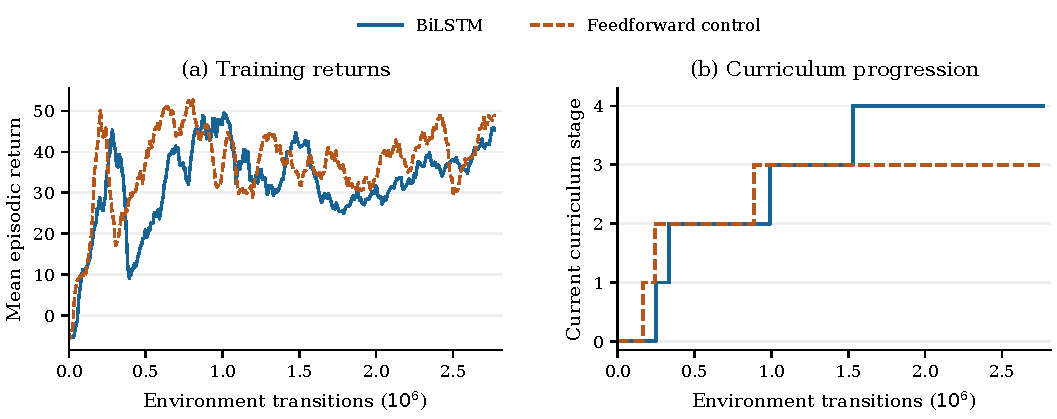
\includegraphics[width=.97\textwidth]{training_curves.pdf}
\caption{Training trajectories under the matched transition budget. (a) Mean episodic return over up to 100 recent completed episodes, including earlier-stage replay; CSV sampling occurs every ten episodes. (b) Current curriculum stage, reconstructed from exact promotion events in the checkpoint records. A stage indicates current training difficulty, not final mastery. Return fluctuations also reflect changing difficulty and replay composition. Each architecture uses one training seed.}
\label{fig:training}
\end{figure*}

Fig.~\ref{fig:training} shows training returns and curriculum progression. The control's final rolling reward, 49.218, exceeds the candidate's 45.355, even though its curriculum progress and stage-4 evaluation are worse. This is consistent with the two windows containing different difficulty mixtures and replay episodes. Raw rolling returns should therefore not rank the architectures directly.

Recorded training throughput is approximately 726 transitions/s for BiLSTM and 1,624 transitions/s for feedforward on the same GPU, a roughly $2.24\times$ throughput advantage for feedforward. These figures summarize the saved runs rather than a dedicated timing benchmark. The control's recorded peak GPU allocation inherits process-level history from the preceding candidate run and should not be interpreted as an independent model-memory measurement. The study compares interaction budgets, not equal wall-clock or compute budgets.

\subsection{Performance Across Curriculum Stages}
Fig.~\ref{fig:success} shows combat success at every evaluation stage. Full-history BiLSTM has higher success than the matched control at all five stages in these trials. Stage-0 success is lower than stage-1 success for each policy despite stage numbering: the stage-0 opponent can fire, and difficulty rules do not imply monotonic outcomes for every learned policy and finite test sample. Exact per-stage values accompany the report in the comparison JSON and raw CSV.

\begin{figure}[t]
\centering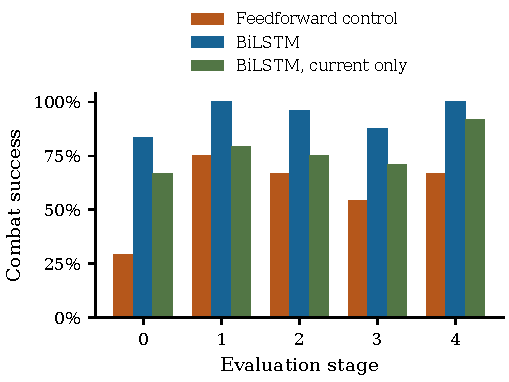
\includegraphics[width=\columnwidth]{stage_success.pdf}
\caption{Combat success under identical evaluation stages, map seeds, and initial spawn seeds. All variants have 24 trials per stage. Current-only uses the full-history policy's weights with a single-observation input.}
\label{fig:success}
\end{figure}

\subsection{Primary Stage-4 Comparison}
On stage 4, BiLSTM succeeds in 24/24 trials, compared with 16/24 for the feedforward control. The observed difference is 33.3 percentage points, with paired bootstrap interval $[16.7,54.2]$ points. Mean reward increases by 21.50, interval $[17.21,25.79]$, and mean kills increase by 2.75, interval $[2.17,3.33]$. Table~\ref{tab:stagefour} includes offensive and defensive measures rather than success alone.

The candidate records 6.46 kills per episode versus 3.71, hit rate 56.5\% versus 34.0\%, and mean damage taken 40.63 versus 76.04. Every candidate episode lasts 1,000 steps, whereas the control averages 892.38 steps. Kills per 1,000 steps are 6.46 versus 4.16, showing that its offensive advantage persists after normalizing for survival duration. Nevertheless, 24/24 observed successes do not imply a true success probability of one on unseen conditions.

\begin{table}[t]
\caption{Stage-4 Matched Evaluation and History Ablation}
\label{tab:stagefour}
\centering\footnotesize
\begin{tabularx}{\columnwidth}{@{}Y r r r@{}}
\toprule Metric & Feedforward & BiLSTM & Current-only \\
\midrule
Combat success & 66.7\% & 100.0\% & 91.7\% \\
Survival & 66.7\% & 100.0\% & 95.8\% \\
Mean reward & 22.67 & 44.17 & 28.92 \\
Mean kills / episode & 3.71 & 6.46 & 4.42 \\
Kills / 1,000 steps & 4.16 & 6.46 & 4.47 \\
Aggregate hit rate & 34.0\% & 56.5\% & 35.5\% \\
Mean damage taken & 76.04 & 40.63 & 53.13 \\
Mean episode length & 892.38 & 1,000.00 & 987.54 \\
\bottomrule
\end{tabularx}
\end{table}

\subsection{What the History Ablation Supports}
With history reduced to one observation, the same BiLSTM weights succeed in 22/24 stage-4 trials, earn 28.92 mean reward, and achieve 4.42 kills per episode. Full history improves reward by 15.25, interval $[10.08,21.00]$, and kills by 2.04, interval $[1.29,2.83]$. Mean damage falls by 12.50, interval $[-21.88,-3.13]$ for full minus current-only.

The success difference is 8.3 percentage points with interval $[0.0,20.8]$. This interval includes zero, so the binary success measure alone does not establish a clear history benefit at that confidence level. Reward and offensive metrics provide stronger evidence of temporal-input sensitivity on these trials. Stage 0 also illustrates metric tradeoffs: the current-only variant has slightly higher reward while full history has higher survival. These observations support a benefit for specific measures under the tested conditions. Recent history may help infer motion and reacquire occluded targets, but the present measurements do not isolate either mechanism.

\subsection{Other Saved Experiments}
Against the separate historical reference, the latest candidate achieves stage-4 success of 100.0\% versus 29.2\%, with rewards 44.17 versus 22.925. The reference uses fewer transitions and unknown original settings. These results must not be substituted for the matched control's 66.7\% success and 22.67 reward.

An earlier two-million-transition scratch run stops at stage 2 and obtains 79.2\% stage-4 success, reward 10.22, against a different historical reference with 70.8\% success and reward 23.46. A still earlier warm-start pilot aggregates two training seeds on evaluation maps 10--13: BiLSTM success is 58.3\%, feedforward continuation success is 31.25\%, and the frozen reference succeeds in 62.5\%. Its reward comparison and saved verdict are inconclusive about a general memory improvement. These pilots demonstrate why survival, kills, reward, initialization, and reference hashes all need explicit reporting. They are not replications of the latest matched study.

\section{Software Verification}
The repository contains 104 test methods across 12 test modules. Tests cover Gymnasium behavior, wall and projectile geometry, angular visibility, variable projectile sets, padding invariance, gradient flow, episode history isolation, exact budgets, checkpoint resume, final-stage qualification, rendering equivalence, reports, and self-play. The test count is a source inventory rather than a claim that every method executes in the current environment.

A recorded headless test run executes 95 discovery entries: 92 pass, one fails, one raises an import error, and one CUDA test skips because CUDA is inaccessible to the process. The missing Streamlit dependency prevents discovery of ten dashboard tests, represented by a single import-error entry. The self-play integration assertion selects a resumed-run CSV through an unsorted directory listing instead of the initial-run report. This reporting check remains unresolved; the suite therefore does not provide a fully passing verification result.


Evaluation verification recomputes every matched stage metric and stored bootstrap interval from all 360 raw episodes, checks checkpoint hashes and parameter counts, and compares the application source with its archived hashes. These checks establish consistency of the saved evidence; they do not constitute a new training run or independent evaluation replication.

\section{Limitations and Future Work}
The primary comparison has one independently trained policy per architecture. More training seeds and new held-out map sets are needed to assess reproducibility. The bootstrap resamples paired trials, not distinct map distributions, and with only four maps it gives limited evidence about generalization. Repeated development on known evaluation maps can also introduce selection bias even when training maps remain disjoint.

The BiLSTM has more parameters and lower throughput. A parameter-matched feedforward control, unidirectional LSTM comparison, multiple context lengths, and equal-compute experiments would help separate temporal information from capacity and optimization effects. The shared adaptive curriculum changes exposure as performance changes. A fixed stage schedule would answer a different question by controlling that exposure explicitly.

The 32-observation window cannot maintain a long-term map or remember an opponent hidden for arbitrarily long periods. Bullets outside the viewing cone remain unobserved, and target velocity must be inferred. Scripted combat also gives the learner faster bullets and a shorter cooldown than its opponent. Human play and symmetric self-play broaden the interface, but the current matched results concern the scripted opponent only. Evaluation against diverse frozen opponents would test whether behaviors transfer beyond that opponent logic.

The history ablation changes the trained input distribution and retains recurrent computation on the current observation. It measures dependence on supplied history, without isolating every cause of the performance difference. Further controls could train one-observation recurrent models from scratch and compare identical capacity under different history availability.

Finally, resume omits simulator/RNG state, dependencies are not fully pinned, and existing dashboard/test issues limit the claim of a completely verified deployment. Archived code, hashes, configuration, and evidence copies improve traceability, but a locked dependency environment and clean verification run would strengthen reproducibility.

\section{Conclusion}
The project implements an inspectable PPO training system for local-observation 2D combat. Angular enemy sectors reduce legacy sensor gaps, a set encoder handles variable visible projectile counts, and bounded recurrence introduces temporal context while preserving the same decision MLP. The shared training engine provides a documented comparison procedure with curriculum qualification and held-out paired trials.

In the saved equal-transition study, BiLSTM completes all five stages and improves stage-4 combat success, reward, kills, accuracy, and damage taken relative to its feedforward control. Removing older observations lowers reward and kills, while the binary success interval remains uncertain. The evidence supports further study of bounded observation history in this environment, with independent training seeds, capacity controls, and broader opponents needed before general architecture claims.

\appendices
\section{Reproducibility and Data Availability}
The primary experiment is stored under
\begin{flushleft}\small
\path{reports/bilstm_gpu_all_stages_20261112/}
\end{flushleft}
The accompanying source package contains raw evaluation episodes, comparison summaries, configuration manifests, training CSVs, and figure-generation code. In the matched records, \code{frozen} identifies the feedforward control. The historical-reference comparison is stored separately. Full checkpoint hashes and parameter counts appear in \path{data/verification.json}; archived application-source hashes match the verified implementation.

The companion \code{BUILD.txt} provides complete training, evaluation, figure-generation, and LaTeX compilation commands. A replication of the adaptive protocol can stop at a different budget. A predeclared-budget experiment should instead train both architectures independently for 2,769,992 transitions with curriculum stopping disabled, then evaluate their checkpoints on the specified held-out trials. Independent training seeds are required to estimate training variability. Supplied figures use the original recorded measurements and include vector PDFs. The application and checkpoints are required to repeat the experiment; the bundled LaTeX and figures suffice to compile the paper.

\bibliographystyle{IEEEtran}
\bibliography{references}
\end{document}
